% !TeX TS-program = luatex

\documentclass[11pt, aspectratio=169]{beamer}

\usetheme{Antibes}
\usecolortheme{seahorse}
\setbeamertemplate{navigation symbols}{}
\setbeamertemplate{headline}{}
\graphicspath{ {./images/} }

% Fonts and emojis
\usepackage{emoji}
\usepackage{fontspec}
\setsansfont{Fira Sans}
\setmonofont{Iosevka}
\usepackage{ulem}

% Codeblocks
\usepackage{minted}
\usemintedstyle{monokai}

% Links coloring
\usepackage{hyperref}
\hypersetup{
	colorlinks=true,
	linkcolor=blue,
	filecolor=magenta,
	urlcolor=blue,
}

\title[Building Helm replacement]{Implementing Your Own Controller with Gateway API}
\author{Denis Shatokhin}
\date{September 2024}

\begin{document}
\maketitle

\begin{frame}{\emoji{card-index-dividers} Table of Content}
	\tableofcontents
\end{frame}

\section{Introduction}

\begin{frame}{\emoji{waving-hand} About Me}
	\begin{description}
		\item [$\bullet$ Devops Engineer (System Administrator)]
		\item [$\bullet$ Work at Relex Solutions]
		\item [$\bullet$ Live in Helsinki for almost 2 years]
		\item [$\bullet$ Really like to build solutions no one asked for]
	\end{description}
\end{frame}

\begin{frame}{\emoji{warning} Disclaimer}
	This is not a production ready solution and was
	built to get more knowledge about \textbf{Gateway API}, \textbf{Apple PKL} and \textbf{Envoy}\\~\\

	\centerline{{\Huge \emoji{smiling-face-with-smiling-eyes}}}
\end{frame}

\section{Ingress vs. Gateway APIs}

\begin{frame}{\emoji{balance-scale} Differences between Ingress and Gateway APIs}
	\begin{tabular}{ |l||l|l| }
		\hline
		                   & \textbf{Ingress} & \textbf{Gateway}                    \\
		\hline\hline
		Protocol support   & HTTP/HTTPS       & L4/L7 support                       \\
		\hline
		Traffic management & Limited          & Built-in advanced support           \\
		\hline
		Portability        & Vendor specifics & Common standard                     \\
		\hline
		Resource objects   & ingress          & gatewayClass, gateway, httpRoute... \\
		\hline
		Routing rules      & Path/host-based  & Path/host/header-based              \\
		\hline
		Extensions         & Annotations      & Part of specification               \\
		\hline
	\end{tabular}
	% \centerline{{\Huge \emoji{heart}}}
\end{frame}

\begin{frame}{\emoji{newspaper} Current state of both APIs}
	\begin{block}{Ingress API}
		Ingress is frozen. New features are being added to the Gateway API\\

		\url{https://kubernetes.io/docs/concepts/services-networking/ingress}
	\end{block}~

	\begin{block}{Gateway API}
		This project represents the next generation of Kubernetes Ingress,
		Load Balancing, and Service Mesh APIs\\

		\url{https://gateway-api.sigs.k8s.io}
	\end{block}~

	The signal is clear – start moving to Gateway API now to migrate smoothly in the future
\end{frame}

\section{Homemade gateway-controller}

\begin{frame}{\emoji{canned-food} Introducing BAGAPI}
	\begin{columns}
		\column{0.6\textwidth}
		\textbf{Bagapi} is a homemade \textbf{gateway controller}\\~\\
		The main idea is to implement \textbf{bare minimum functionality}.\\~\\
		Should be written in bash logic mounted to pod via \textbf{configmap}.\\~\\

		The configuration for proxy stored in \textbf{configmap} as well.\\~\\

		\textbf{Bagapi} is a successor of \textbf{Bashgress} --
		ingress-controller with \textbf{bash} and \textbf{jq} under the hood:

		\url{https://github.com/dshatokhin/bashgress}

		\column{0.4\textwidth}
		
\includegraphics[width=\textwidth]{bagapi.png}
	\end{columns}
\end{frame}

\begin{frame}{\emoji{thinking-face} How It Works}
	The main component manually deployed to cluster is \textbf{bagapi-provisioner}:

	\begin{description}
		\item [$\bullet$ uses \textbf{kubectl} to get all \textbf{gateway} objects in cluster in \textbf{json} format]
		\item [$\bullet$ uses \textbf{pkl} to parse \textbf{gateway.json} file]
		\item [$\bullet$ outputs \textbf{k8s} manifests for \textbf{controller} and \textbf{envoy}]
	\end{description}~

	The \textbf{controller} automatically deployed for every \textbf{gateway} object in the cluster:

	\begin{description}
		\item [$\bullet$ uses \textbf{kubectl} to get all \textbf{HTTProute} objects in cluster in \textbf{json} format]
		\item [$\bullet$ uses \textbf{pkl} to parse \textbf{httproutes.json} file]
		\item [$\bullet$ outputs \textbf{configmap} which \textbf{envoy} reading]
		\item [$\bullet$ \textbf{envoy} reads mounted files contained in \textbf{configmap}]
		\item [$\bullet$ \textbf{envoy} dynamicly gets changes via file-based xDS]
	\end{description}~

	Also, the \textbf{service} with \textbf{type: Loadbalancer} created for every \textbf{gateway} object.
\end{frame}

\begin{frame}[label=demopicture]{\emoji{framed-picture} How It Works}
	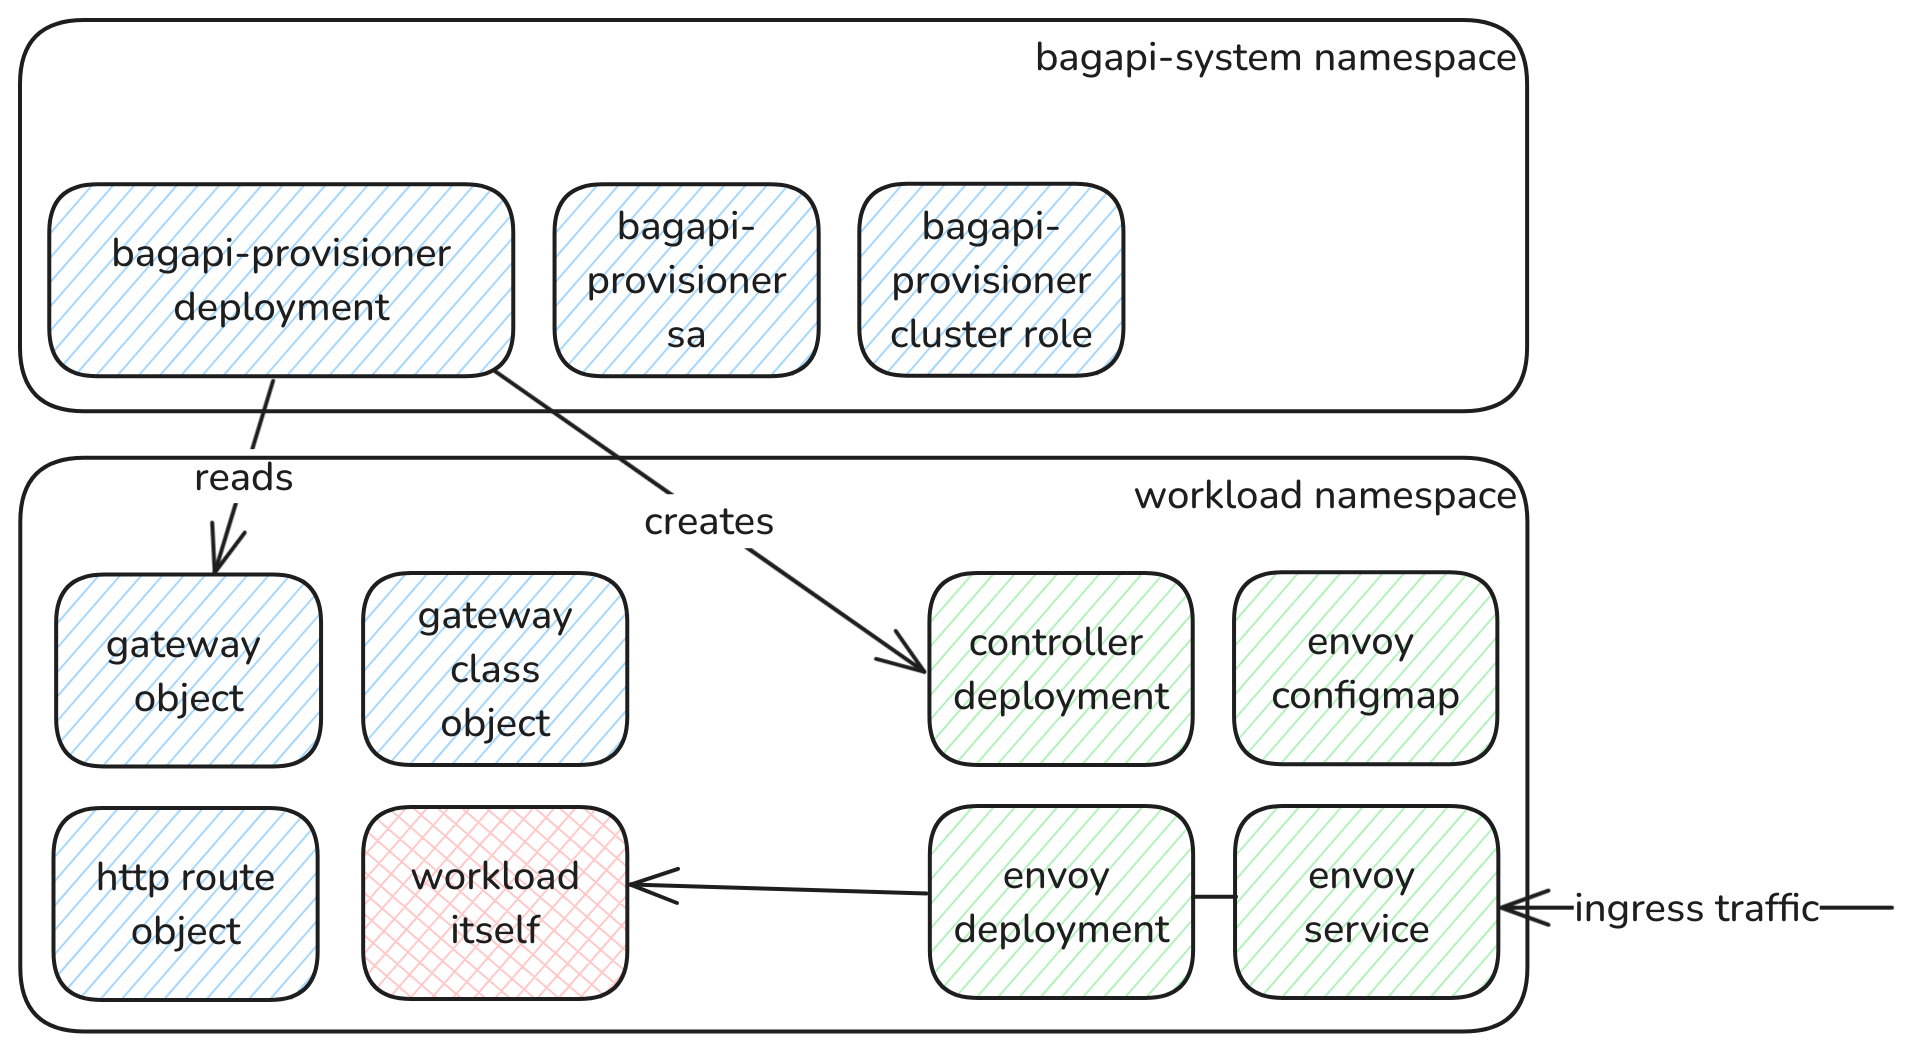
\includegraphics[width=0.95\textwidth]{scheme.png}
\end{frame}

\begin{frame}{\emoji{up-down-arrow} Envoy}
	Build by LYFT, \textbf{v1.0.0} released back in \textbf{2016}.
	From the official documentation:

	\begin{block}{quote}
		Envoy is an L7 proxy and communication bus designed for large modern service oriented architectures.
		The project was born out of the belief that:
		\begin{description}
			\item [$\bullet$ The network should be transparent to applications]
			\item [$\bullet$ When network and application problems do occur it]
			\item [$\bullet$ should be easy to determine the source of the problem]
		\end{description}
	\end{block}

	\begin{description}
		\item [$\bullet$ L3/L4 - TCP/UDP, HTTP, TLS, custom protocols like
		      \textbf{postgres}, \textbf{redis}, \textbf{kafka} etc]
		\item [$\bullet$ HTTP L7 - buffering, rate limiting, routing/forwarding]
		\item [$\bullet$ HTTP/1.1, HTTP/2, HTTP/3 support]
		\item [$\bullet$ service discovery and \textbf{dynamic configuration} (xDS)]
		\item [$\bullet$ really good observability]
		\item [$\bullet$ could be extended via \textbf{LUA} or \textbf{WASM}]
		\item [$\bullet$ written in \textbf{C++}]
	\end{description}
\end{frame}

\begin{frame}{\emoji{cucumber} Apple Pkl}
	\textit{pronounced Pickle}\\~\\
	Build by Apple and open-sourced earlier this year:

	\begin{block}{quote}
		Pkl -- is an embeddable configuration language which provides rich support
		for data templating and validation. It can be used from the command line,
		integrated in a build pipeline, or embedded in a program. Pkl scales
		from small to large, simple to complex, ad-hoc to repetitive configuration tasks.
	\end{block}

	\begin{description}
		\item [$\bullet$ turing complete]
		\item [$\bullet$ written in \textbf{java}]
		\item [$\bullet$ LSP support on the corner]
		\item [$\bullet$ community growing fast]
		\item [$\bullet$ no Apple ID required]
	\end{description}
\end{frame}

\section{Demo}

\begin{frame}{\emoji{crossed-fingers} Demo}
	Let's see how it works\\~\\
	\centerline{{\Huge \emoji{smirking-face}}}
\end{frame}

\section{Questions}

\begin{frame}{\emoji{link} Links}
	Code and presentation:
	\begin{description}
		\item [$\bullet$ \href{https://github.com/dshatokhin/bagapi}{github.com/dshatokhin/bagapi}]
		\item [$\bullet$ \href{https://github.com/dshatokhin/presentations}{github.com/dshatokhin/presentations}]
	\end{description}~

	Additional links:
	\begin{description}
		\item [$\bullet$ \href{https://gateway.envoyproxy.io}{gateway.envoyproxy.io}
		      -- Envoy-gateway - envoy-based gateway-controller]
		\item [$\bullet$ \href{https://pkl-lang.org}{pkl-lang.org}
		      -- Apple PKL]
		\item [$\bullet$ \href{https://www.envoyproxy.io}{www.envoyproxy.io}
		      -- Envoy]
		\item [$\bullet$ \href{https://gateway-api.sigs.k8s.io/implementations}{gateway-api.sigs.k8s.io/implementations}
		      -- List of gateway-controllers]
	\end{description}
\end{frame}

\begin{frame}{\emoji{red-question-mark} Questions}
	If you have any...
\end{frame}
\end{document}
